\documentclass[12pt,a4paper]{article}

% --- Pacotes Fundamentais ---
\usepackage[utf8]{inputenc}
\usepackage[T1]{fontenc}
\usepackage[portuguese]{babel}
\usepackage{graphicx}       % Para incluir imagens
\usepackage{geometry}       % Para ajustar margens
\usepackage{amsmath}        % Para fórmulas matemáticas avançadas
\usepackage{float}          % Para posicionamento de figuras
\usepackage{hyperref}       % Para links clicáveis
\usepackage{booktabs}       % Para tabelas bonitas
\usepackage{longtable}      % Para tabelas longas
\usepackage{array}          % Para melhor controle de tabelas
\usepackage{indentfirst}    % Indenta o primeiro parágrafo
\usepackage{setspace}       % Para controle de espaçamento entre linhas

% --- Configuração de Espaçamento Matemático ---
\setlength{\jot}{15pt} 

% --- Configuração das Molduras das Imagens ---
\setlength{\fboxsep}{6pt}  % Espaço entre a imagem e a moldura (o recuo)
\setlength{\fboxrule}{0.5pt} % Espessura da linha da moldura

% --- Configuração de Links ---
\hypersetup{
	colorlinks=true,
	linkcolor=black,
	filecolor=magenta,      
	urlcolor=blue,
}

% --- Margens ---
\geometry{left=3cm, top=3cm, right=2cm, bottom=2cm}

\begin{document}
	
	% --- CAPA PERSONALIZADA ---
	\begin{titlepage}
		\begin{center}
			% --- Área dos Logos (SEM MOLDURA) ---
			\begin{figure}[h]
				\centering
				
\includegraphics[height=1.3cm]{../images/softex.png} \hspace{1cm}
				
\includegraphics[height=1.3cm]{../images/cpqd.png} \hspace{1cm}
				
\includegraphics[height=1.3cm]{../images/fiap.png}
			\end{figure}
			
			\vspace{1.5cm}
			
			% --- Cabeçalho Institucional ---
			\large \textbf{MCTI/SOFTEX + CPQD + FIAP} \\
			\large Programa de Especialização/Residência em Sistemas Eletrônicos Embarcados \\
			
			\vfill 
			
			% --- Título do Projeto ---
			\Huge \textbf{Projeto Prático nº 3} \\[0.5cm]
			\Large \textbf{Sistema de Forno IoT}
			
			\vfill
			
			% --- Autores ---
			\large \textbf{Matheus Grossi} \\
			\large \textbf{Talles Mello} \\
			\large \textbf{Manassés Loiola} \\
			\large \textbf{Helton Abadia}
			
			\vspace{1cm}
			
			% --- Links de Acesso Rápido ---
			\noindent\rule{8cm}{0.4pt} \\ 
			\vspace{0.3cm}
			\small \textbf{Acesso Rápido ao Projeto:} \\
			\href{https://wokwi.com/projects/454130082230099969}{Simulação no Wokwi} $\bullet$ 
			\href{https://stem.ubidots.com/app/dashboards/69701418221d689174891929}{Dashboard Ubidots} $\bullet$ 
			\href{https://github.com/IOT-Eletric-Oven-FIAP/fiap_embedded_project_iot_eletric_oven}{Repositório GitHub}
			
			\vfill
			
			% --- Local e Data ---
			\large Campinas, SP \\ 2026
			
		\end{center}
	\end{titlepage}
	
	% --- Sumário ---
	\tableofcontents
	\newpage
	
	% --- Conteúdo ---
	
	\section{Objetivos}
	
	O sistema simula um forno com conectividade IoT. O ESP32 realiza as seguintes funções principais:
	\begin{itemize}
		\item Ler a temperatura do sensor NTC.
		\item Ler o potenciômetro (referência do usuário), que pode ser usado como setpoint (temperatura-alvo) ou potência/PWM diretamente (duty cycle).
		\item Com o forno habilitado pelo botão, calcular a saída e acionar o LED (representando a resistência).
		\item Publicar periodicamente os dados via MQTT (ex.: temperatura, referência, estado do forno e saída).
		\item Exibir informações no display (integrado ao circuito).
	\end{itemize}
	
	\section{Descrição do Projeto}
	
	Este trabalho objetivou a criação de um sistema de forno elétrico IoT, contemplando:
	\begin{itemize}
		\item \textbf{Conectividade:} Implementação de um broker que centraliza os dados e fornece um dashboard.
		\item \textbf{Interface Homem-Máquina (IHM):} Desenvolvimento de uma interface a partir do display LCD 320x240 (IL9341), simplificando a centralização visual dos dados.
		\item \textbf{Controle:} Leitura de sensores analógicos e acionamento de carga (LED PWM) baseado em referências de usuário.
	\end{itemize}
	
	\section{Dimensionamento e Lista de Materiais}
	
	\subsection{Cálculo do Resistor para os LEDs}
	Serão utilizados dois LEDs neste contexto: o \textbf{amarelo} (simula iluminação externa/relé) e um \textbf{vermelho} (luz de alerta/GPIO).
	O cálculo baseia-se na tensão máxima do GPIO do ESP32 ($V_{pp} = 3.3V$).
	
	\subsubsection{Fórmulas Utilizadas}
	\begin{enumerate}
		\item \textbf{Resistência Mínima Segura:}
		\[ R(\Omega) = \frac{V_{pp} - V_{led}}{I_{led}} \]
		
		\item \textbf{Dissipação de Potência:}
		\[ P(W) = U \cdot i \]
		
		\item \textbf{Potência Mínima do Resistor (Fator de Segurança $Fs = 50\%$):}
		\[ P_{min} = P(W) \cdot (1 + Fs) \]
	\end{enumerate}
	
	\begin{figure}[H]
		\centering
		% \fbox{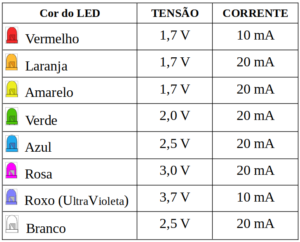
\includegraphics[width=0.8\textwidth]{../images/tabela_led.png}}
		\caption{Tabelas de referência para LEDs e Resistores (Consultar anexos)}
	\end{figure}
	
	\subsection{Dimensionamento Aplicado}
	
	Abaixo demonstram-se os cálculos efetuados para a definição dos componentes.
	
	\subsubsection{LED Vermelho}
	Dados: $V_{led} \approx 1.7V$, $I_{led} = 10mA$ ($0.01A$).
	\begin{align*}
		R &= \frac{3.3 - 1.7}{0.01} = \frac{1.6}{0.01} = 160\Omega \\
		P &= 1.6 \cdot 0.01 = 0.016W \\
		P_{min} &= 0.016 \cdot 1.5 = 0.024W
	\end{align*}
	
	\textbf{Conclusão:} Valor comercial adotado de \textbf{160R}.
	Potência comercial mais próxima: \textbf{1/16W} (0.0625W).
	
	\subsubsection{LED Amarelo}
	Dados: $V_{led} \approx 1.7V$, $I_{led} = 20mA$ ($0.02A$).
	\begin{align*}
		R &= \frac{3.3 - 1.7}{0.02} = \frac{1.6}{0.02} = 80\Omega \\
		P &= 1.6 \cdot 0.02 = 0.032W \\
		P_{min} &= 0.032 \cdot 1.5 = 0.048W
	\end{align*}
	
	\textbf{Conclusão:} Valor comercial adotado de \textbf{82R} (arredondamento).
	Potência comercial mais próxima: \textbf{1/16W} (0.0625W).
	
	\section{Lista de Materiais (BOM)}
	
	Abaixo, a relação dos componentes utilizados na aplicação:
	
	\begin{table}[H]
		\centering
		\begin{tabular}{ll}
			\toprule
			\textbf{Item} & \textbf{Descrição} \\ \midrule
			Microcontrolador & ESP32-S3-DEVKITC-1-N8R8 \\
			Display & LCD 20x4 (com fundo azul) \\
			Sensor & Sensor de temperatura NTC-10K \\
			Entrada & Push-Button (Chave Tátil 6x6x6mm) \\
			Iluminação & LED Difuso 5mm Vermelho \\
			Resistor & 160R 1/16W \\
			Resistor & 82R 1/16W \\
			Entrada & Potenciômetro Linear 10kR \\ \bottomrule
		\end{tabular}
		\caption{Lista de Materiais Utilizados}
	\end{table}
	
	\section{Critérios de Projeto e Pinagem}
	
	\subsection{Mapeamento de I/Os (Pinout)}
	O mapa de conexões adotado para o ESP32-S3-DEVKITC-1-N8R8 é detalhado abaixo.
	
	\begin{longtable}{|c|p{12cm}|}
		
		\hline
		\textbf{GPIO} & \textbf{Função} \\ \hline
		\endfirsthead
		
		\hline
		\textbf{GPIO} & \textbf{Função} \\ \hline
		\endhead
		
		\hline
		\multicolumn{2}{|r|}{\small Continua...} \\ \hline
		\endfoot
		
		\endlastfoot
		
		4 & Entrada Digital: Push-Button \\ \hline
		11 & Entrada Analógica: Sensor de temperatura NTC \\ \hline
		12 & Entrada Analógica: Potenciômetro \\ \hline
		14 & Saída Digital: Controle PWM (LED) \\ \hline
		36 & Entrada Digital (SPI): TFT - MISO \\ \hline
		38 & Saída Digital (SPI): TFT - SCK \\ \hline
		39 & Saída Digital (SPI): TFT - MOSI \\ \hline
		40 & Saída Digital (SPI): TFT - DC \\ \hline
		41 & Saída Digital (SPI): TFT - RST \\ \hline
		42 & Saída Digital (SPI): TFT - CS \\ \hline
		
		\noalign{\vspace{10pt}} 
		\caption{Mapa de Conexões do Microcontrolador}
		
	\end{longtable}
	
	\begin{figure}[H]
		\centering
		\fbox{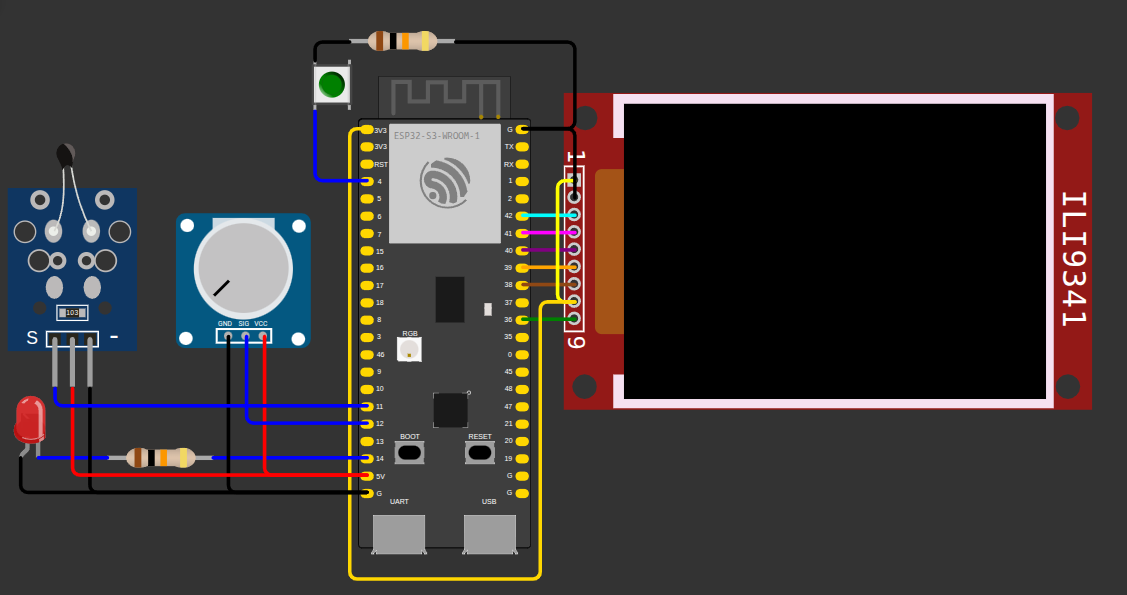
\includegraphics[width=0.8\textwidth]{../images/ope_tel_0.png}}
		\caption{Diagrama Visual das Conexões}
	\end{figure}
	
	\subsection{Sequência de Inicialização (Boot)}
	
	O sistema possui uma sequência visual de inicialização no display TFT. Abaixo seguem as telas capturadas:
	
	\begin{figure}[H]
		\centering
		\fbox{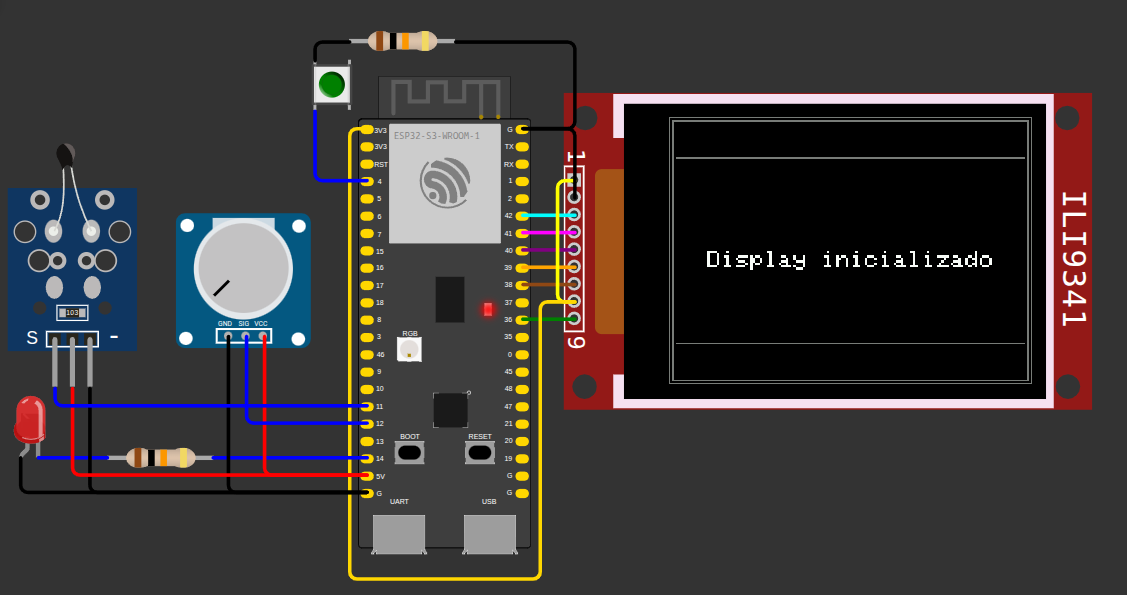
\includegraphics[width=0.7\textwidth]{../images/ope_tel_1.png}}
		\caption{Estágio 1: Inicialização do Display}
	\end{figure}
	
	\begin{figure}[H]
		\centering
		\fbox{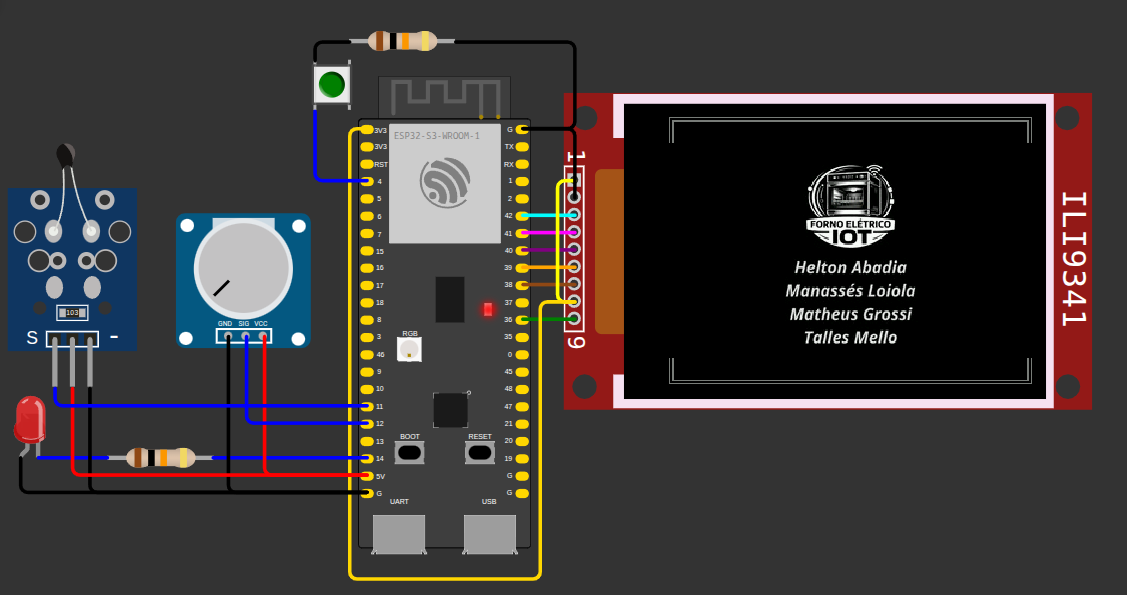
\includegraphics[width=0.7\textwidth]{../images/ope_tel_2.png}}
		\caption{Estágio 2: Escopo do Projeto}
	\end{figure}
	
	\begin{figure}[H]
		\centering
		\fbox{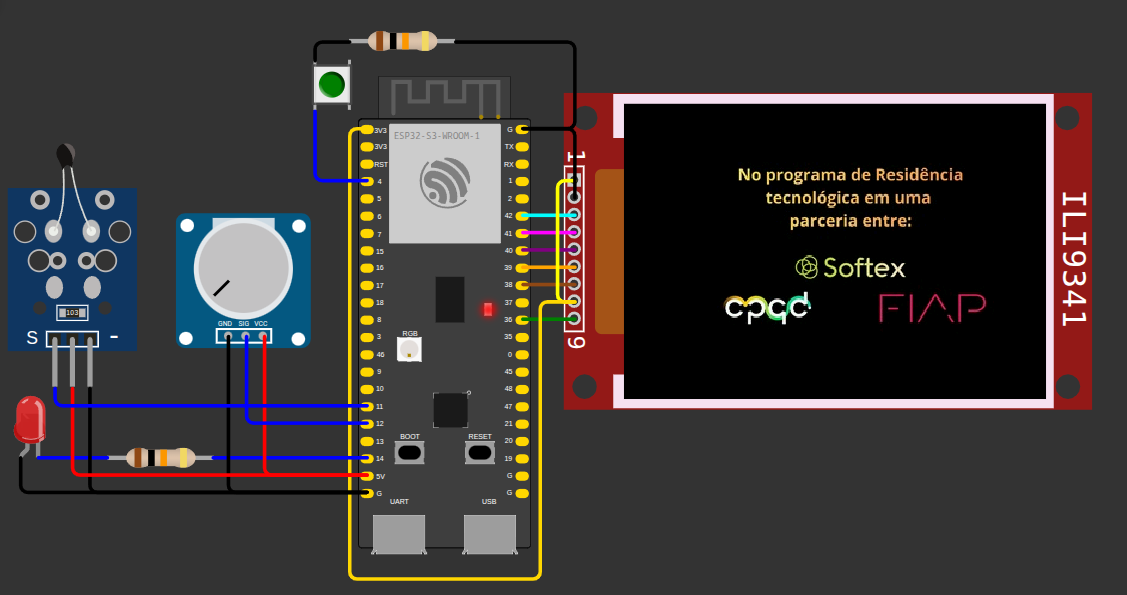
\includegraphics[width=0.7\textwidth]{../images/ope_tel_3.png}}
		\caption{Estágio 3: Créditos}
	\end{figure}
	
	\begin{figure}[H]
		\centering
		\fbox{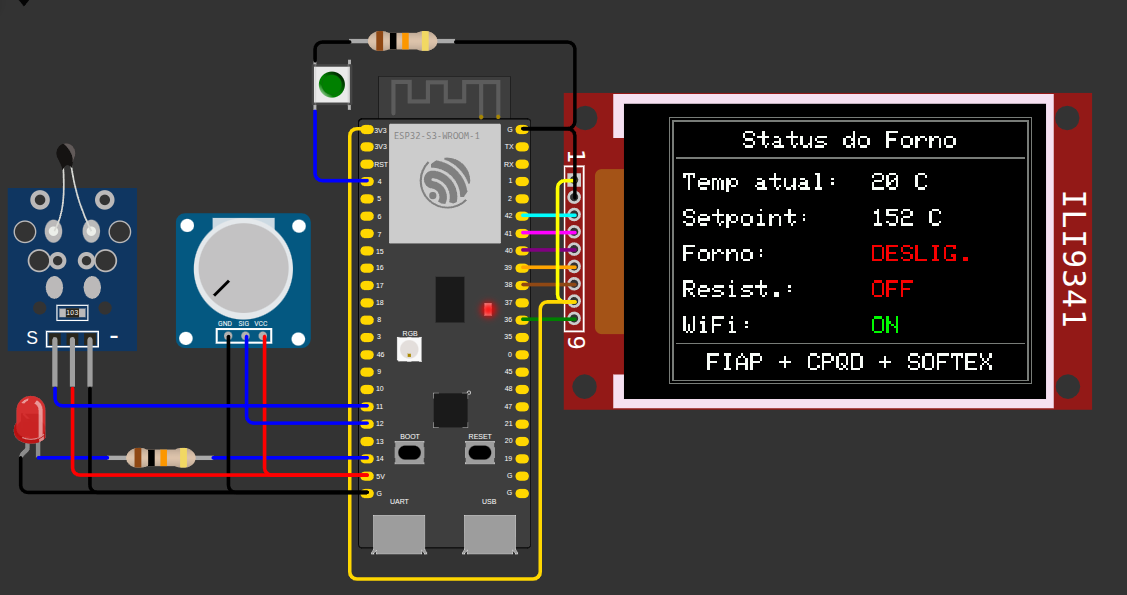
\includegraphics[width=0.7\textwidth]{../images/ope_tel_4.png}}
		\caption{Regime Permanente: Tela de Operação}
	\end{figure}
	
	\section{Arquitetura do Firmware}
	
	A estrutura de arquivos do projeto está organizada da seguinte forma:
	
	\begin{table}[H]
		\centering
		\begin{tabular}{|p{5cm}|p{10.5cm}|}
			\hline
			\textbf{Arquivo} & \textbf{Função} \\ \hline
			\texttt{main.cpp} & Processamento principal e execução das funções primárias. \\ \hline
			\texttt{wifi.cpp} & Centraliza comandos para conexão Wi-Fi. \\ \hline
			\texttt{http.cpp} & Centraliza comandos para conexão ao broker (HTTP/MQTT). \\ \hline
			\texttt{tft.cpp} & Suporte ao display TFT LCD IL9341. \\ \hline
			\texttt{img1.cpp} & Cabeçalho de inicialização 1 (Imagem convertida). \\ \hline
			\texttt{img2.cpp} & Cabeçalho de inicialização 2 (Imagem convertida). \\ \hline
			\texttt{tft.h} & Header de funções recursivas de conexão ao display. \\ \hline
			\texttt{http.h} & Header de funções recursivas de conexão ao HTTP. \\ \hline
		\end{tabular}
		\caption{Estrutura de Arquivos do Firmware}
	\end{table}
	
	\section{Resultados e Interação}
	
	A implementação permitiu o monitoramento via dashboard das grandezas do sistema.
	O funcionamento foi validado através da captura de dados e visualização gráfica no ThingSpeak/Ubidots.
	
	\begin{figure}[H]
		\centering
		\fbox{\includegraphics[width=0.8\textwidth]{../images/dash_1.png}}
		\caption{Dashboard em operação}
	\end{figure}
	
\end{document}